%!TeX root=../pridetop.tex
\chapter[Chapter \thechapter]{}
	
	
\begin{figure}[t!]
\centering

\includegraphics[width=.6\linewidth]{40top}
\captionlistentry{Headpiece to Chapter \thechapter}
\end{figure}


\lettrine[lines=6,image=true]{initials/chap40e}{lizabeth's} impatience to acquaint Jane with what had happened could no longer be overcome; and at length resolving to suppress every particular in which her sister was concerned, and preparing her to be surprised, she related to her the next morning the chief of the scene between Mr Darcy and herself.

\zz
Miss Bennet's astonishment was soon lessened by the strong sisterly partiality which made any admiration of Elizabeth appear perfectly natural; and all surprise was shortly lost in other feelings. She was sorry that Mr Darcy should have delivered his sentiments in a manner so little suited to recommend them; but still more was she grieved for the unhappiness which her sister's refusal must have given him.

»His being so sure of succeeding was wrong,« said she, »and certainly ought not to have appeared; but consider how much it must increase his disappointment.«

»Indeed,« replied Elizabeth, »I am heartily sorry for him; but he has other feelings which will probably soon drive away his regard for me. You do not blame me, however, for refusing him?«

»Blame you! Oh, no.«

»But you blame me for having spoken so warmly of Wickham?«

»No—I do not know that you were wrong in saying what you did.«

»But you \textit{will} know it, when I have told you what happened the very next day.«

She then spoke of the letter, repeating the whole of its contents as far as they concerned George Wickham. What a stroke was this for poor Jane, who would willingly have gone through the world without believing that so much wickedness existed in the whole race of mankind as was here collected in one individual! Nor was Darcy's vindication, though grateful to her feelings, capable of consoling her for such discovery. Most earnestly did she labour to prove the probability of error, and seek to clear one, without involving the other.

»This will not do,« said Elizabeth; »you never will be able to make both of them good for anything. Take your choice, but you must be satisfied with only one. There is but such a quantity of merit between them; just enough to make one good sort of man; and of late it has been shifting about pretty much. For my part, I am inclined to believe it all Mr Darcy's, but you shall do as you choose.«

It was some time, however, before a smile could be extorted from Jane.

»I do not know when I have been more shocked,« said she. »Wickham so very bad! It is almost past belief. And poor Mr Darcy! dear Lizzy, only consider what he must have suffered. Such a disappointment! and with the knowledge of your ill opinion too! and having to relate such a thing of his sister! It is really too distressing, I am sure you must feel it so.«

»Oh no, my regret and compassion are all done away by seeing you so full of both. I know you will do him such ample justice, that I am growing every moment more unconcerned and indifferent. Your profusion makes me saving; and if you lament over him much longer, my heart will be as light as a feather.«

»Poor Wickham! there is such an expression of goodness in his countenance! such an openness and gentleness in his manner.«

»There certainly was some great mismanagement in the education of those two young men. One has got all the goodness, and the other all the appearance of it.«

»I never thought Mr Darcy so deficient in the \textit{appearance} of it as you used to do.«

»And yet I meant to be uncommonly clever in taking so decided a dislike to him, without any reason. It is such a spur to one's genius, such an opening for wit, to have a dislike of that kind. One may be continually abusive without saying anything just; but one cannot be always laughing at a man without now and then stumbling on something witty.«

»Lizzy, when you first read that letter, I am sure you could not treat the matter as you do now.«

»Indeed, I could not. I was uncomfortable enough, I was very uncomfortable—I may say unhappy. And with no one to speak to of what I felt, no Jane to comfort me, and say that I had not been so very weak, and vain, and nonsensical, as I knew I had! Oh, how I wanted you!«

»How unfortunate that you should have used such very strong expressions in speaking of Wickham to Mr Darcy, for now they \textit{do} appear wholly undeserved.«

»Certainly. But the misfortune of speaking with bitterness is a most natural consequence of the prejudices I had been encouraging. There is one point on which I want your advice. I want to be told whether I ought, or ought not, to make our acquaintance in general understand Wickham's character.«

Miss Bennet paused a little, and then replied, »Surely there can be no occasion for exposing him so dreadfully. What is your own opinion?«

»That it ought not to be attempted. Mr Darcy has not authorized me to make his communication public. On the contrary, every particular relative to his sister was meant to be kept as much as possible to myself; and if I endeavour to undeceive people as to the rest of his conduct, who will believe me? The general prejudice against Mr Darcy is so violent, that it would be the death of half the good people in Meryton, to attempt to place him in an amiable light. I am not equal to it. Wickham will soon be gone; and, therefore, it will not signify to anybody here what he really is. Some time hence it will be all found out, and then we may laugh at their stupidity in not knowing it before. At present I will say nothing about it.«

»You are quite right. To have his errors made public might ruin him for ever. He is now, perhaps, sorry for what he has done, and anxious to re-establish a character. We must not make him desperate.«

The tumult of Elizabeth's mind was allayed by this conversation. She had got rid of two of the secrets which had weighed on her for a fortnight, and was certain of a willing listener in Jane, whenever she might wish to talk again of either. But there was still something lurking behind, of which prudence forbade the disclosure. She dared not relate the other half of Mr Darcy's letter, nor explain to her sister how sincerely she had been valued by his friend. Here was knowledge in which no one could partake; and she was sensible that nothing less than a perfect understanding between the parties could justify her in throwing off this last encumbrance of mystery. »And then,« said she, »if that very improbable event should ever take place, I shall merely be able to tell what Bingley may tell in a much more agreeable manner himself. The liberty of communication cannot be mine till it has lost all its value!«

She was now, on being settled at home, at leisure to observe the real state of her sister's spirits. Jane was not happy. She still cherished a very tender affection for Bingley. Having never even fancied herself in love before, her regard had all the warmth of first attachment, and from her age and disposition, greater steadiness than first attachments often boast; and so fervently did she value his remembrance, and prefer him to every other man, that all her good sense, and all her attention to the feelings of her friends, were requisite to check the indulgence of those regrets which must have been injurious to her own health and their tranquillity.

\begin{figure}[h!]
\centering
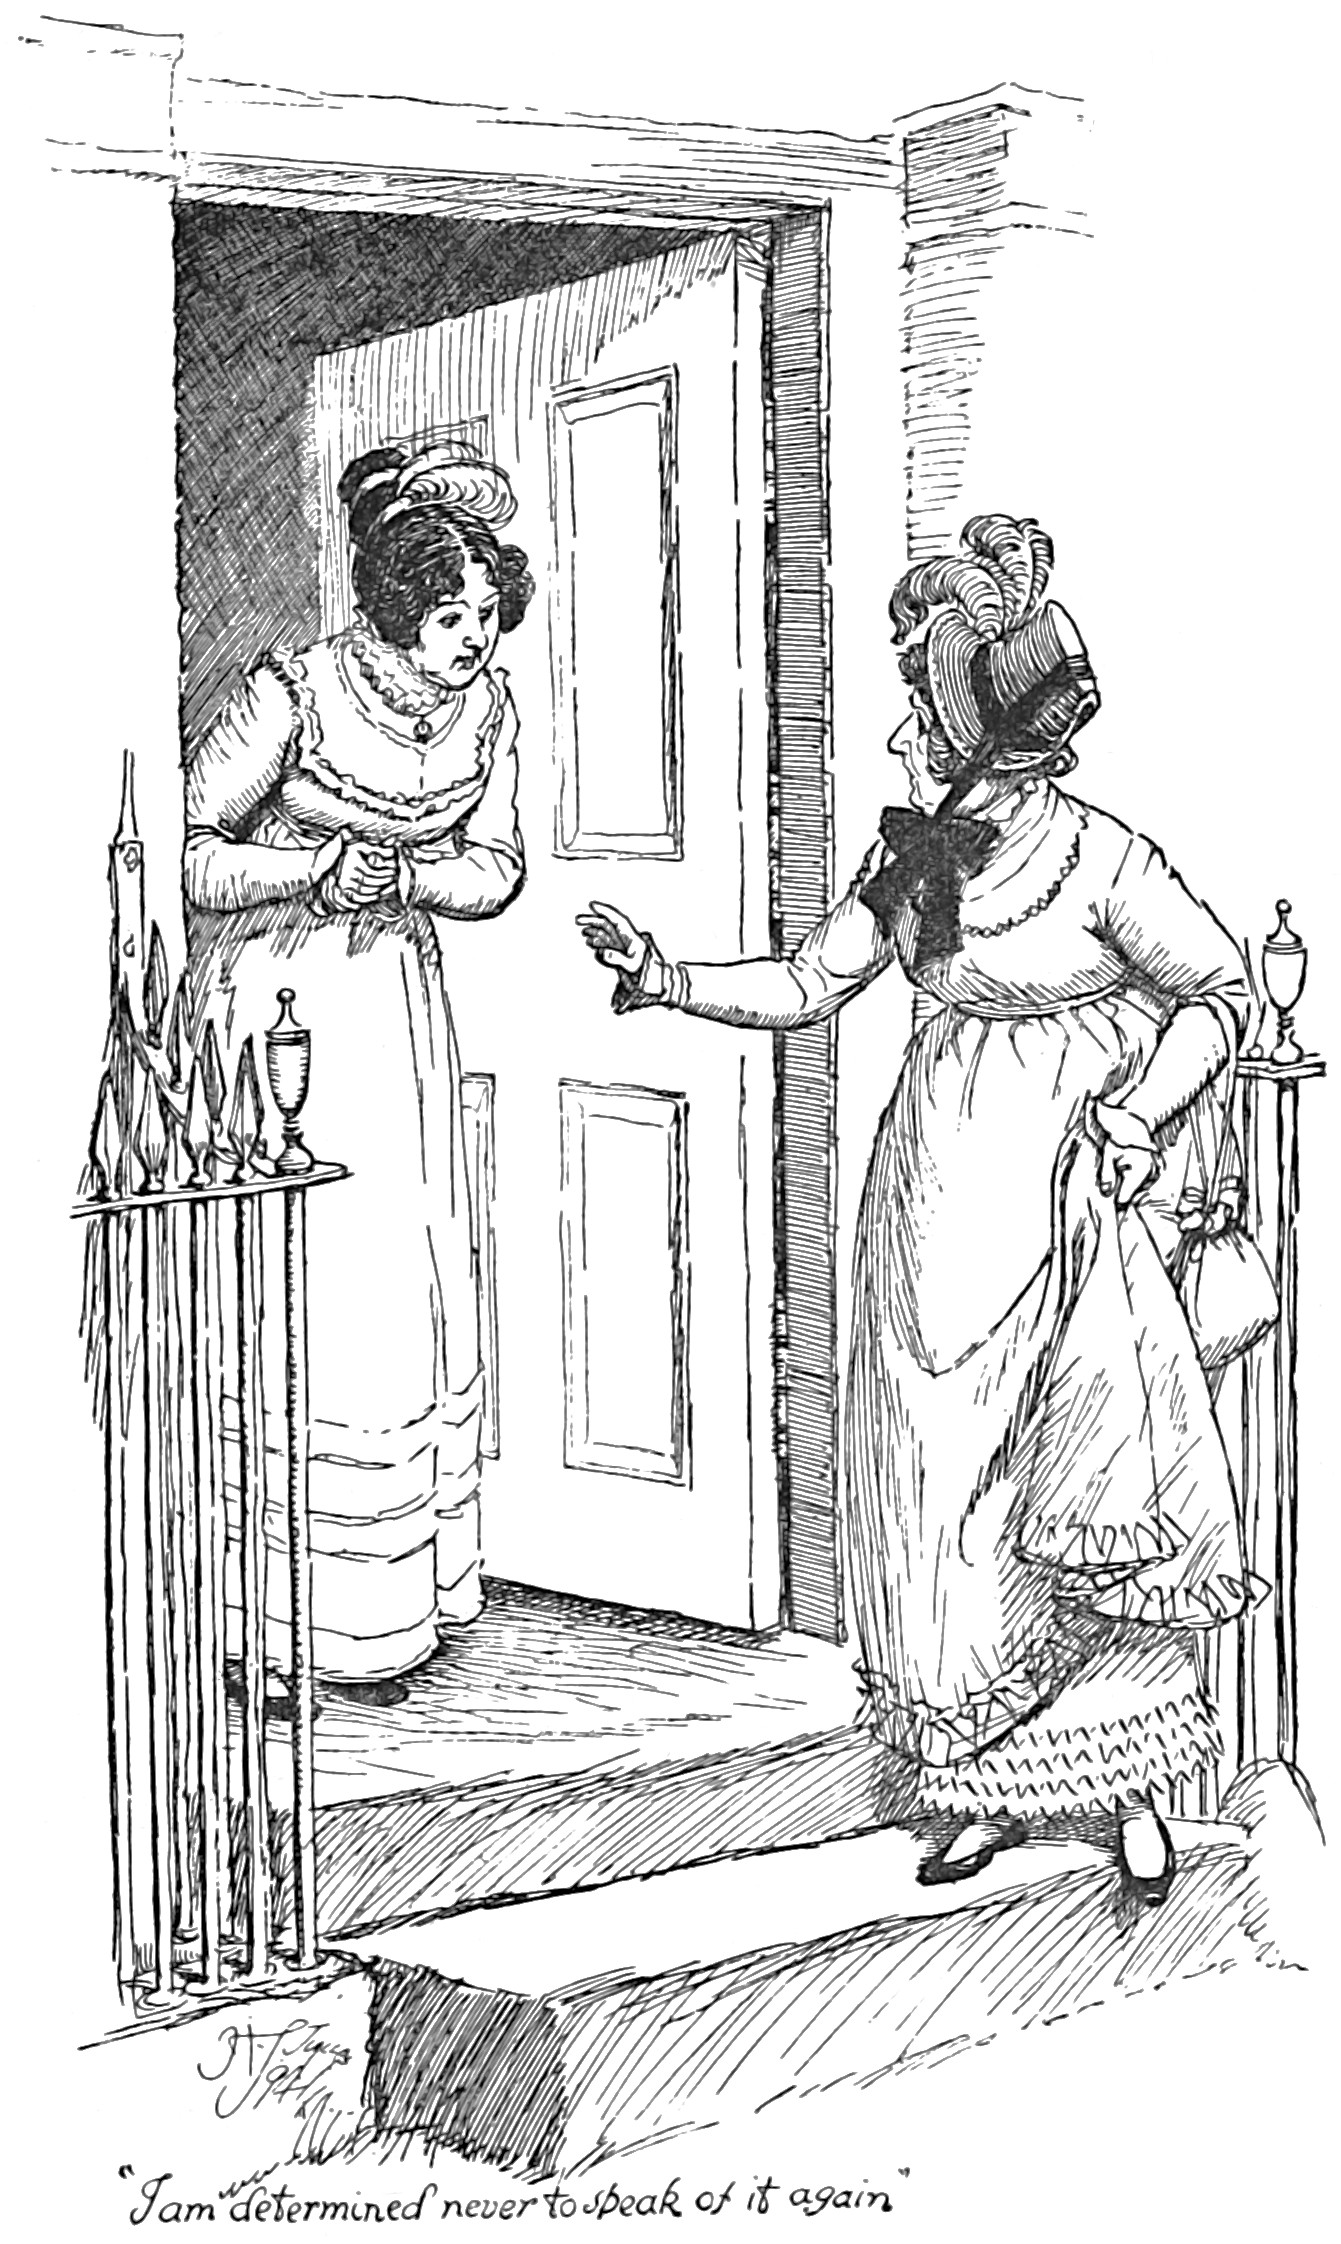
\includegraphics[width=.8\linewidth]{40speak}
\captionlistentry{»I am determined never to speak of it again«}
\end{figure}

»Well, Lizzy,« said Mrs Bennet, one day, »what is your opinion \textit{now} of this sad business of Jane's? For my part, I am determined never to speak of it again to anybody. I told my sister Philips so the other day. But I cannot find out that Jane saw anything of him in London. Well, he is a very undeserving young man—and I do not suppose there is the least chance in the world of her ever getting him now. There is no talk of his coming to Netherfield again in the summer; and I have inquired of everybody, too, who is likely to know.«

»I do not believe that he will ever live at Netherfield any more.«

»Oh, well! it is just as he chooses. Nobody wants him to come; though I shall always say that he used my daughter extremely ill; and, if I was her, I would not have put up with it. Well, my comfort is, I am sure Jane will die of a broken heart, and then he will be sorry for what he has done.«

But as Elizabeth could not receive comfort from any such expectation she made no answer.

»Well, Lizzy,« continued her mother, soon afterwards, »and so the Collinses live very comfortable, do they? Well, well, I only hope it will last. And what sort of table do they keep? Charlotte is an excellent manager, I dare say. If she is half as sharp as her mother, she is saving enough. There is nothing extravagant in \textit{their} housekeeping, I dare say.«

»No, nothing at all.«

»A great deal of good management, depend upon it. Yes, yes. \textit{They} will take care not to outrun their income. \textit{They} will never be distressed for money. Well, much good may it do them! And so, I suppose, they often talk of having Longbourn when your father is dead. They look upon it quite as their own, I dare say, whenever that happens.«

»It was a subject which they could not mention before me.«

»No; it would have been strange if they had. But I make no doubt they often talk of it between themselves. Well, if they can be easy with an estate that is not lawfully their own, so much the better. \textit{I} should be ashamed of having one that was only entailed on me.«